\documentclass[week2]{csse1001}

\title{CSSE1001 Week 5 Practicals}
 
\begin{document}

\begin{frame} 
\maketitle
\end{frame}

\section{Some assignment dos and don'ts...}

\begin{topic}{Bad: Global variables}
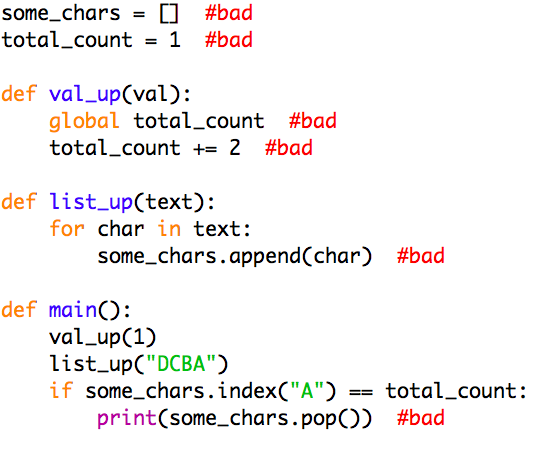
\includegraphics[height=0.9\textheight]{bad_python/globals}
\end{topic}

\begin{topic}{Good: Use of constants}
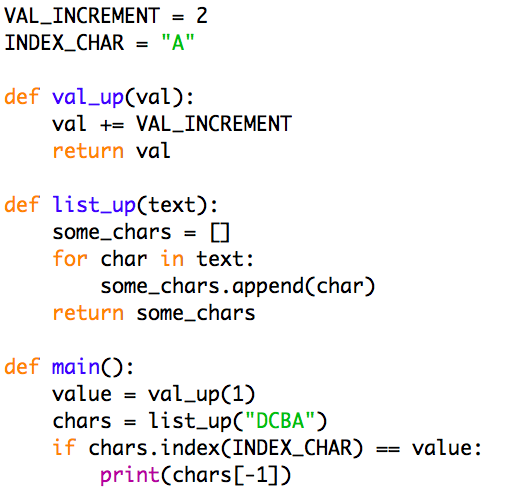
\includegraphics[height=0.9\textheight]{bad_python/constants}
\end{topic}

\begin{topic}{Bad: Lazy variable naming}
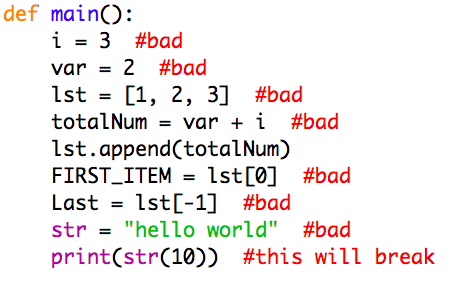
\includegraphics[height=0.8\textheight]{bad_python/bad_naming}
\end{topic}

\begin{topic}{Good: Meaningful variable names}
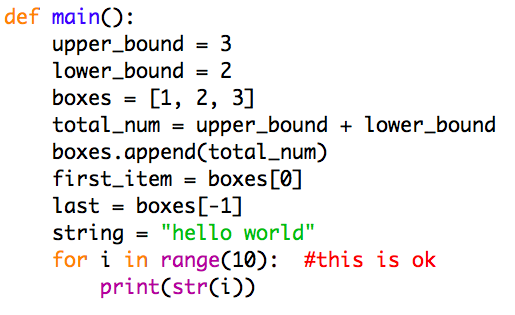
\includegraphics[height=0.8\textheight]{bad_python/good_naming}
\end{topic}

\begin{topic}{Bad: Lengthy functions}
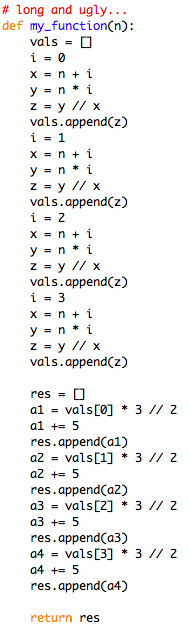
\includegraphics[height=0.9\textheight]{bad_python/long}
\end{topic}

\begin{topic}{Good: Functional decomposition and use of control structures}
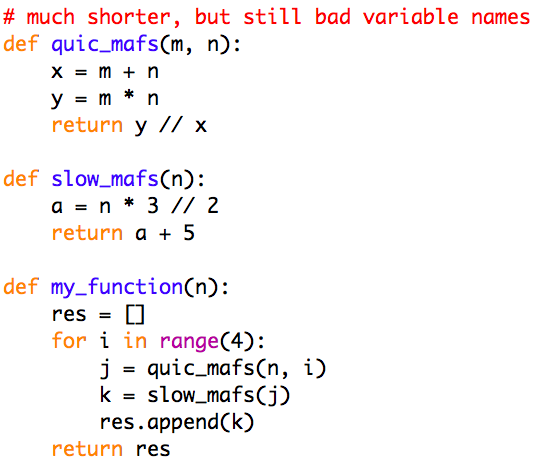
\includegraphics[height=0.9\textheight]{bad_python/short}
\end{topic}

\begin{topic}{Bad: Not following the spec}
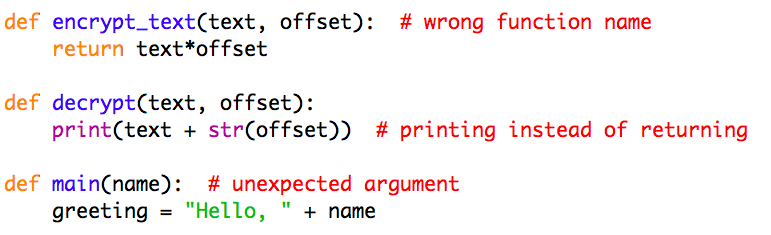
\includegraphics[height=0.4\textheight]{bad_python/incorrect}

(note that the implementations are completely absurd...)
\end{topic}

\begin{topic}{Good: Following the spec exactly}
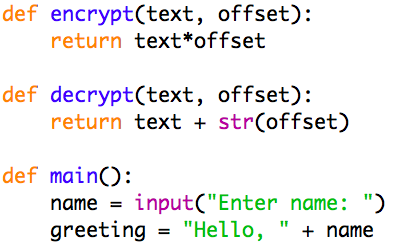
\includegraphics[height=0.6\textheight]{bad_python/correct}

(note that the implementations are completely absurd...)
\end{topic}

\begin{topic}{Bad: No documentation}
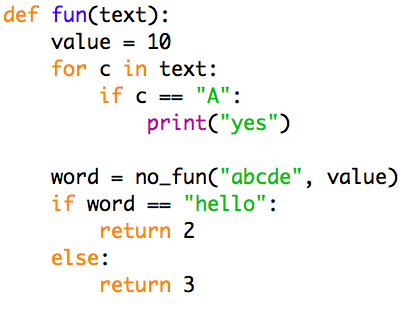
\includegraphics[height=0.9\textheight]{bad_python/no_comments}
\end{topic}

\begin{topic}{Also Bad: Overcommenting}
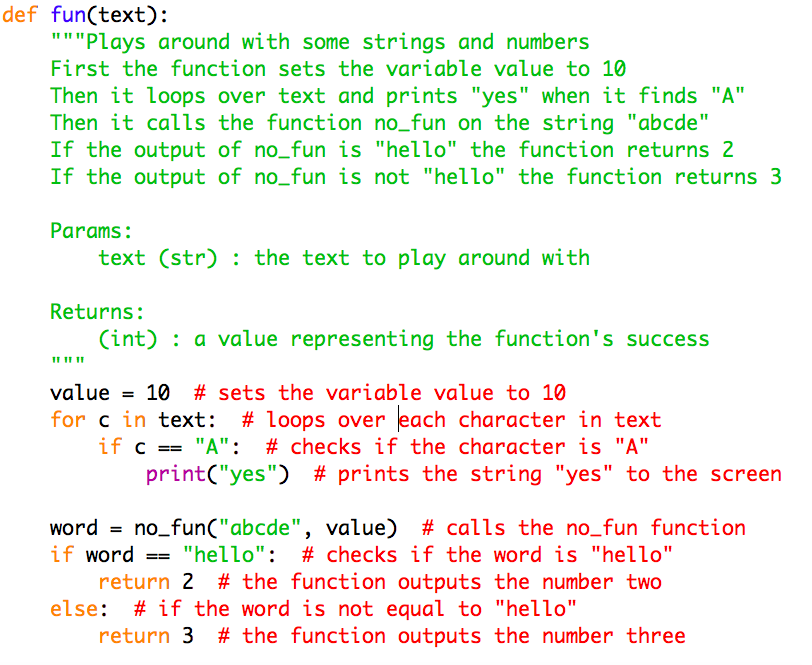
\includegraphics[height=0.9\textheight]{bad_python/bad_comments}
\end{topic}

\begin{topic}{Good: Appropriate docstrings and comments}
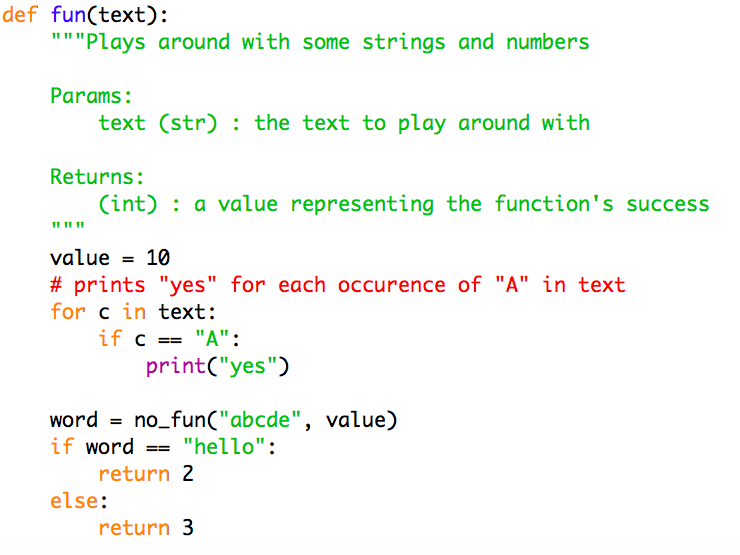
\includegraphics[height=0.9\textheight]{bad_python/good_comments}
\end{topic}

\section{Sample tests}

\begin{topic}{Example output}
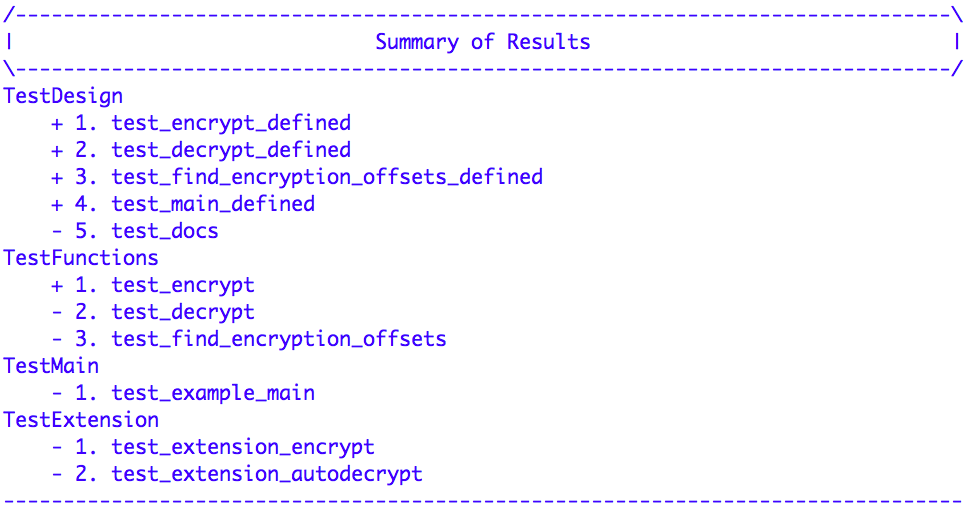
\includegraphics[height=0.9\textheight]{testsa1/overview}
\end{topic}

\begin{topic}{Interpreting failures}
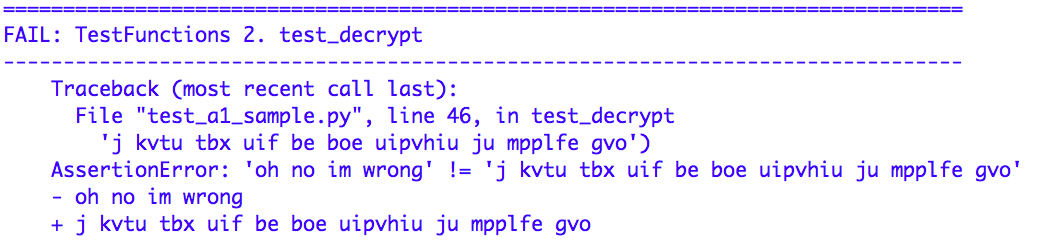
\includegraphics[height=0.9\textheight]{testsa1/fail}
\end{topic}

\begin{topic}{Interpreting failures}
Make sure your output is \textit{exact}!

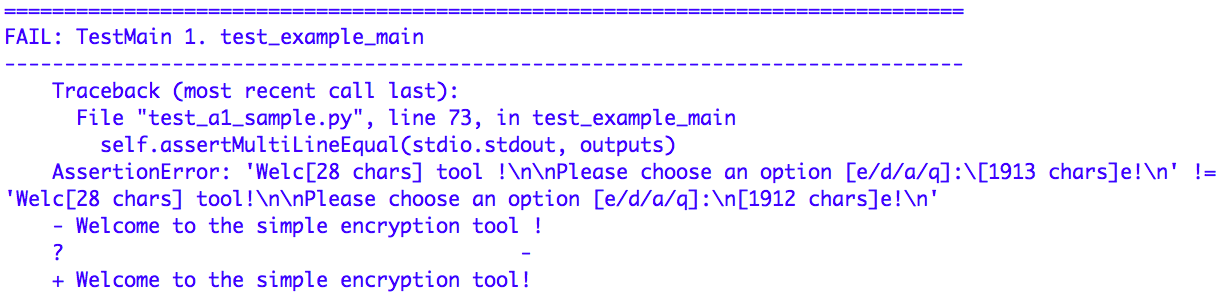
\includegraphics[height=0.8\textheight]{testsa1/fail2}
\end{topic}

\section{Reminder: Assignment is due this Friday at 8:30pm!}

\end{document} 
